% !TEX root = ../main.tex

\begin{savequote}[99mm]
Let us change our traditional attitude to the construction of programs: Instead of imagining that our main task is to instruct a computer what to do, let us concentrate rather on explaining to human beings what we want a computer to do.\qauthor{Donald Knuth}
\end{savequote}

\chapter{Identification problem}\label{chap:id-problem}

Cellular Automata (CAs) constitute an attractive and effective modeling paradigm for a variety of problems~\cite{das2012}. In order to use CAs for a practical modeling task, one needs to understand the mechanisms underlying the phenomenon at stake, and translate them into a CA rule. Additionally, the state space and neighborhood structure need to be pinned down beforehand. This limits the use of CAs, since there are problems for which manually designing a local rule is hard. Moreover, in some cases only the initial and final states of the system are known (\emph{e.g.}~\cite{urban-ga,pattern-ga,image-proc}). Research on automated CA identification is motivated by such problems. Various methods have been studied so far in this field: Genetic Algorithms (GAs)~\cite{richards1990extracting,mitchell1996evolving,foo01,Sapin:2003:RCA:1762668.1762709}, genetic programming~\cite{conf/automata/BandiniMV08,DBLP:journals/jca/MaedaS07,andre1996discovery}, gene expression programming~\cite{DBLP:journals/corr/cs-AI-0102027}, other evolutionary algorithms~\cite{lukas2018}, ant colony algorithms~\cite{Liu:2008:BAD:1459980.1459984},  machine learning approaches~\cite{DBLP:journals/jca/BullA07}, as well as direct construction algorithms~\cite{adamatzky1994identification,journals/tsmc/YangB00,Yang:2000:NDR:2229236.2229683,Sun11}. Within these methods, two main groups can be identified. Firstly, there are methods for solving specific, global problems. An example of such a problem is the density classification problem in which only the initial condition and the desired outcome is known~\cite{gacs1978one,packard1988adaptation,1751-8121-50-34-345103,Dembowski2017}. Secondly, there are methods that exploit the entire time series of configurations. Typically, it is assumed that all configurations are known (\emph{i.e.}\ observed completely). Only limited  efforts have been devoted to solve the identification problem in the absence of complete information~\cite{richards1990extracting}.

The main goal of the research presented in this paper is to design a method capable of automated CA identification in the case of incomplete information. The incompleteness of the information, within the scope of this paper, is of a~twofold nature. Firstly, we consider \emph{spatial incompleteness}, which relates to missing states of specific cells at one or more time stamps. Secondly, we consider \emph{temporal incompleteness}, which relates to missing CA configurations at certain time stamps. In contrast to spatial incompleteness, where the location and therefore the amount of missing information is known, these parameters are not known in the case of temporal incompleteness, \emph{i.e.}\ a certain, unknown number of time stamps are missing in between every consecutive pair of observed time stamps. Such a setting has not yet been discussed in the literature. In this paper, a detailed definition of this identification problem is presented. Moreover, an effective solution algorithm based on a GA is presented.

It is important to understand the motivation behind the problem definition discussed in this paper. Essentially, spatial incompleteness can be related to malfunctioning measuring equipment or limited capabilities of observing real-world phenomena. Such scenarios are very likely in many practical applications~\cite{chuvieco2009fundamentals}. Temporal incompleteness, on the other hand, can be understood in two ways. Firstly, similarly to spatial incompleteness, it can be related to limited observation capabilities, \emph{i.e.}\ the frequency of capturing the time stamps might be limited and unstable. Secondly, there is the issue of synchronization. The clock of the phenomenon in question, and the one of the prospective CA-based model, are not necessarily in synchrony. Due to this, the number of CA time stamps in between two consecutive observed time stamps might be unknown and might be changing dynamically. Consequently, although the problem is discussed in a theoretical setting of 1D, two-state CAs, the nature of the tackled problems relates directly to the one of practical modelling.

In this chapter, we introduce the identification problem. Our formulation is based on the concept of an incomplete observation of a space-time diagram, \emph{i.e.}\ it contains only incomplete information on the states of the underlying~CA.

Let $I \in \{0,1,?\}^{N\times M}$. We interpret $I$ as an array containing symbols from the set $\{0,1,?\}$. The role of the symbol~``?'' is to indicate that information on the actual state of a cell is lacking. Additionally, let the first row $I[1]$ be completely observed, \emph{i.e.}\ $I[1]\in\{0,1\}^M$. We will refer to such an array $I$ as an \emph{observation}. An observation $I\in \{0,1\}^{N\times M}$, \emph{i.e.}\ an observation that does not contain the symbol~``?'', will be called \emph{spatially complete}.

Note that the assumption of a completely observed first row is crucial for the construction of the presented algorithm and cannot be relaxed easily. Yet, in many practical applications there might be natural means of controlling the initial state, for example by repeating laboratory experiments multiple times, thus this assumption can be easily met.

\begin{example}
	We will visualize observations as space-time diagrams where the cells of the configurations are colored white if their state is 0 and black when it is 1, while grey is used to color cells whose state is unknown. Following this convention, Fig.~\ref{fig:ex-obs-comp} shows a complete observation, in this case a space-time diagram of ECA 57. In Fig.~\ref{fig:ex-obs-spat} some of the states in the complete space-time diagram of ECA 57 are changed to ``?'', resulting in a spatially incomplete observation. Finally, Fig.~\ref{fig:ex-obs-temporal} depicts an observation, where some of the states are changed to ``?'' and some configurations are omitted from the complete space-time diagram, resulting in a temporally incomplete observation.\qed%
	\begin{figure*}
		\centering
		\subfloat[]{\fbox{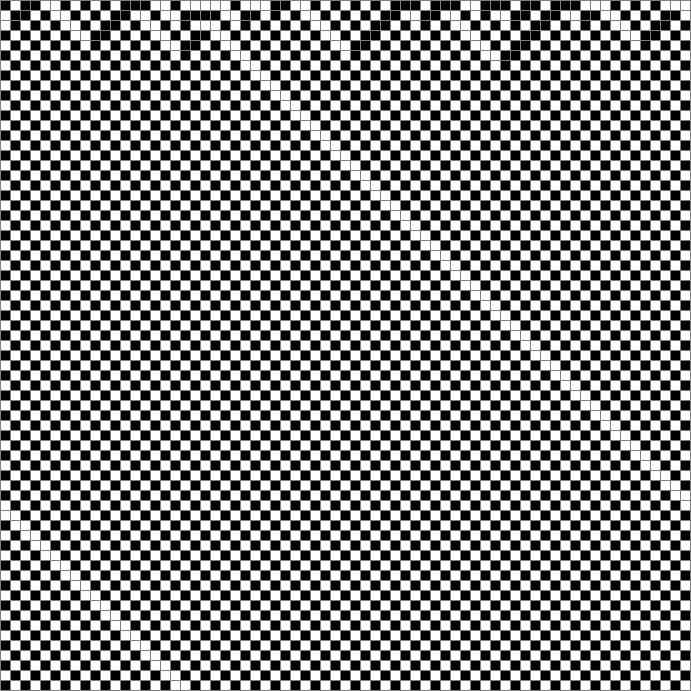
\includegraphics[width=.29\textwidth]{figs/rule-57-01-clear.png}}\label{fig:ex-obs-comp}}\quad
		\subfloat[]{\fbox{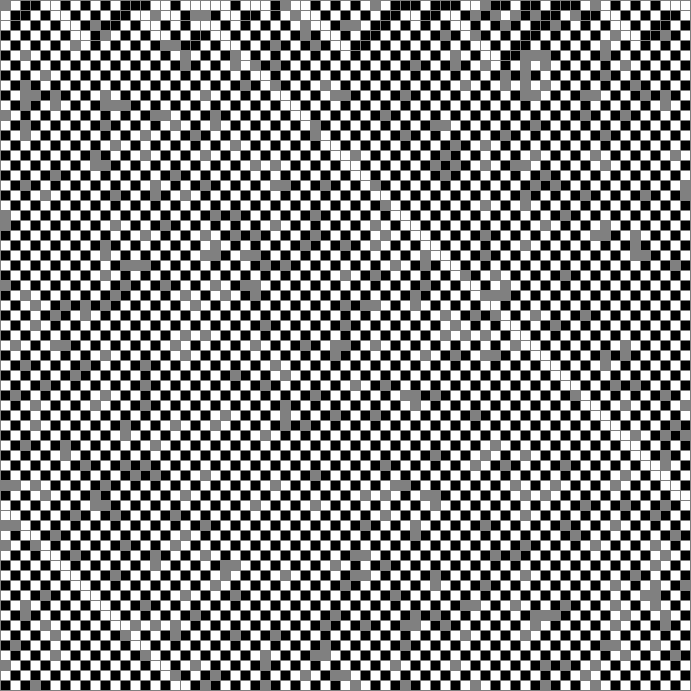
\includegraphics[width=.29\textwidth]{figs/rule-57-02-spatial.png}}\label{fig:ex-obs-spat}}\quad
		\subfloat[]{\fbox{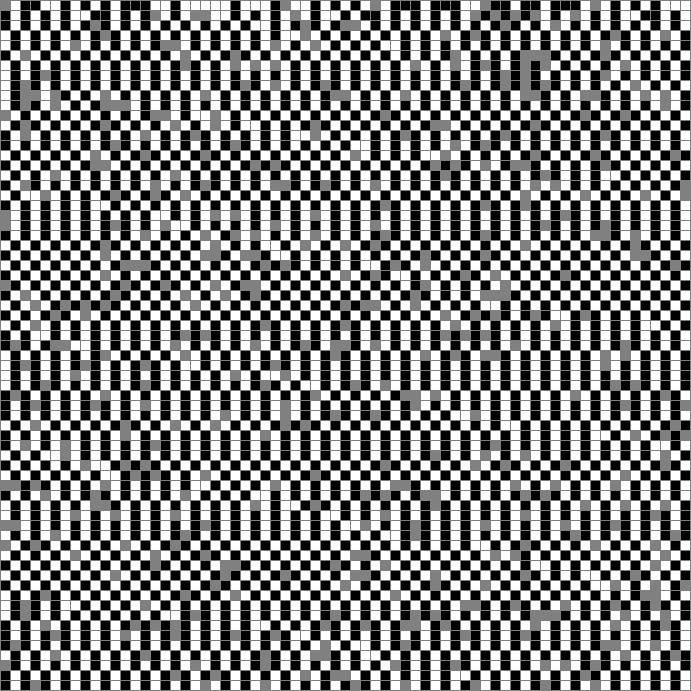
\includegraphics[width=.29\textwidth]{figs/rule-57-03-time.png}}\label{fig:ex-obs-temporal}}
		\caption{Observations of ECA 57 in (\protect\subref*{fig:ex-obs-comp}) complete, (\protect\subref*{fig:ex-obs-spat}) spatially incomplete and (\protect\subref*{fig:ex-obs-temporal}) spatially and temporally incomplete form.}\label{fig:ex-obs}
	\end{figure*}
\end{example}

Let $I$ be an observation. The number of completely observed states is defined as $C(I) = \#\{I[n,m]\neq{}?\}$. In our setting, it holds that $C(I)\geq M$, due to the assumption that $I[1]\in\{0,1\}^M$. With a given observation~$I$, we associate the set $\com(I)$ of all of the spatially complete observations $I'$ satisfying $I'[n,m] = I[n,m]$ for all $n$, $m$ such that $I[n,m]\neq{}?$.
\begin{fact}
\label{fac:count}
For any observation $I$, it holds that $\abs{\com(I)}=2^{N M-C(I)}$.
\end{fact}

\begin{example}
\label{ex:i}
Consider the observation $I$ given by:
\[
I = \begin{array}{|c|c|c|}
\hline
0 & 1 & 0  \\ \hline
0 & {\pmb ?} & 1  \\ \hline
1 & 1 & {\pmb ?} \\ \hline
\end{array}
\]
Since $C(I)=7$, the set $\com(I)$ contains four elements:
\begin{align*}
\com(I) = \left\{ 
\begin{array}{|c|c|c|}
\hline
0 & 1 & 0 \\ \hline
0 & {\pmb 0} & 1  \\ \hline
1 & 1 & {\pmb 0}  \\ \hline
\end{array}\,,
\begin{array}{|c|c|c|}
\hline
0 & 1 & 0  \\ \hline
0 & {\pmb 0} & 1  \\ \hline
1 & 1 & {\pmb 1}  \\ \hline
\end{array}\,,
\begin{array}{|c|c|c|}
\hline
0 & 1 & 0  \\ \hline
0 & {\pmb 1} & 1  \\ \hline
1 & 1 & {\pmb 0}  \\ \hline
\end{array}\,,
\begin{array}{|c|c|c|}
\hline
0 & 1 & 0  \\ \hline
0 & {\pmb 1} & 1  \\ \hline
1 & 1 & {\pmb 1} \\ \hline
\end{array}
\right\}.\tag*{\qed}
\end{align*}
\end{example}

We will say that a CA $A$ \emph{fits an observation $I$} if there exists an $I'\in\com(I)$ and an increasing sequence of positive natural numbers $\sigma = (\sigma_i)_{i=1}^{N-1}$ such that for any $n\in\{1,2,\dotsc,N-1\}$:
\begin{equation}
	A^{\sigma_n}(I'[1]) = I'[n+1]\,.
	\label{eq:fitting}
\end{equation}
The meaning of a CA $A$ fitting an observation $I$, is that the rows of $I$ correspond to configurations of $A$ at some time stamps, which are given by $\sigma$. The first row corresponds to the initial configuration. Entries with the symbol ``?'' correspond to unknown states. Examining $I'$, which is easy to obtain once $A$ and $\sigma$ are found, allows to uncover these unknown states.

\begin{prop}\label{prop:alternative-prob}
	A CA $A$ fits an observation $I$ if and only if there exist an $I'\in\com(I)$ and a sequence of natural numbers $\gamma = (\gamma_i)_{i=1}^{N-1}$ such that for any $n\in\{1,2,\dotsc,N-1\}$:
	\begin{equation}
		A^{1+\gamma_n}(I'[n]) = I'[n+1]\,.
	\end{equation}
\end{prop}

The sequence $\sigma=(\sigma_i)_{i=1}^{N-1}$ in~\eqref{eq:fitting} corresponds to the time stamps in the CA evolution (which are assigned to the rows of the observation), while the sequence $\gamma = (\gamma_i)_{i=1}^{N-1}$ in Proposition~\ref{prop:alternative-prob} refers to the time gaps, \emph{i.e.}\ the number of missing time stamps between two consecutive rows in the observed diagram. Obviously, $\sigma_{n} = \sum_{i=1}^n (1+\gamma_i)$.

\begin{example}
	Consider the following space-time diagram $D$. It shows the evolution of ECA 150 from a single black cell. For the sake of readability, rows have been labelled with the corresponding time stamps.
	\[
		\begin{array}{|c|c|c|c|c|c|c|c|c|l}
			\cline{1-9}
			0 & 0 & 0 & 0 & 1 & 0 & 0 & 0 & 0 & t=0 \\\cline{1-9}
			0 & 0 & 0 & 1 & 1 & 1 & 0 & 0 & 0 & t=1 \\\cline{1-9}
			0 & 0 & 1 & 0 & 1 & 0 & 1 & 0 & 0 & t=2 \\\cline{1-9}
			0 & 1 & 1 & 0 & 1 & 0 & 1 & 1 & 0 & t=3 \\\cline{1-9}
			1 & 0 & 0 & 0 & 1 & 0 & 0 & 0 & 1 & t=4 \\\cline{1-9}
		\end{array}
	\]
	Let the observation $I$ be given by:
	\[
		\begin{array}{|c|c|c|c|c|c|c|c|c|l}\cline{1-9}
			0 & 0 & 0 & 0 & 1 & 0 & 0 & 0 & 0 & t = 0  \\\cline{1-9}
			0 & 1 & 1 & ? & ? & 0 & 1 & 1 & 0 & t ={}? \\\cline{1-9}
			1 & ? & 0 & 0 & ? & 0 & 0 & 0 & ? & t ={}? \\\cline{1-9}
		\end{array}
	\]
	We see that the space-time diagram $D$ and observation $I$ share the same initial configuration, \emph{i.e.}\ $D[1] = I[1]$.
	Now, let $I'\in\com(I)$ be given by:
	\[
		\begin{array}{|c|c|c|c|c|c|c|c|c|l}\cline{1-9}
			0 & 0 & 0 & 0 & 1 & 0 & 0 & 0 & 0 & t = 0  \\\cline{1-9}
			0 & 1 & 1 & 0 & 1 & 0 & 1 & 1 & 0 & t ={}? \\\cline{1-9}
			1 & 0 & 0 & 0 & 1 & 0 & 0 & 0 & 1 & t ={}? \\\cline{1-9}
		\end{array}
	\]
	It holds that $D[4] = I'[2]$ and $D[5] = I'[3]$. We know that $A(D[4]) = D[5]$, since $D$ is the space-time diagram of a CA $A$, and so $A(I'[2]) = I'[3]$. Additionally, it holds that $A^3(D[1]) = D[4] = I'[2]$. Since $I'[1] = D[1]$, it holds that $A^3(I'[1])~=~I'[2]$. According to Proposition~\ref{prop:alternative-prob}, this means that CA $A$ fits the observation $I$.\qed%
\end{example}

In practice, we want to use multiple observations to complete the identification task. Therefore, we will consider a finite set of observations $\mathcal{I}$.
%For simplicity, we assume that the elements of $\mathcal{I}$ are numbered, \emph{i.e.}\ $\mathcal{I} =\{I_1,\dotsc,I_{\abs{\mathcal{I}}}\}$. 
We will say that rule $A$ fits the observation set $\mathcal{I}$ if it fits all of the observations contained in this set. We will write $C(\mathcal{I})$ to express the number of observed states in all of the observations belonging to $\mathcal{I}$, \emph{i.e.}\ $C(\mathcal{I}) = \sum_{I\in\mathcal{I}} C(I)$. Moreover, we will use $M_\mathcal{I}$ to denote the total number of columns in the observations belonging to this observation set, \emph{i.e.}\ $M_\mathcal{I} = \sum_{I\in\mathcal{I}} M_I$, where $M_I$ is the number of columns in observation $I$. We will denote the number of rows $N_I$ in an observation $I\in\mathcal{I}$ by $N_I$. For an observation set $\mathcal{I}$, the set $\rules(\mathcal{I})$ denotes the set of all CAs fitting the observation set $\mathcal{I}$. With the above definitions,  we can restate the identification problem as finding all (or some) of the elements of the set $\rules(\mathcal{I})$. In this paper, we will restrict this formulation of the identification problem to finding at least one of the elements of the set $\rules(\mathcal{I})$.

The following fact will be used in the design of the identification algorithm in order to reduce the computational burden by considering only subsets of the observation set for the calculation of the error, as such enabling a fast method for estimating the values of the fitness function (this approach is described in detail in Section~\ref{sec:fitness}). Informally, this fact can be understood by considering the set $\mathcal{I}$ as the set of conditions that a rule needs to meet. Having fewer conditions, it becomes more likely to find solutions. Yet, no solutions are omitted by relaxing the conditions.

\begin{fact}
	Let $\mathcal{I}$ and $\mathcal{I}'$ be observation sets such that $\mathcal{I}'\subseteq \mathcal{I}$. Then $\rules(\mathcal{I})\subseteq\rules(\mathcal{I}')$.\label{fac:rules-set}
\end{fact}

We consider only finite observation sets, therefore, we know that for every observation set $\mathcal{I}$ there exists a $\Gamma>0$ which is a common upper bound for all of the time gaps in all observations belonging to $\mathcal{I}$. In other words, if a solution to the identification problem exists, and $\gamma^I$ is the sequence of time gaps of observation $I\in\mathcal{I}$, then $0\leq \gamma^I_n\ < \Gamma$, for every $I\in\mathcal{I}$ and $n~=~1,\dotsc,N_I-1$.
In the remainder, it is assumed that the upper bound $\Gamma$ is known. Hence, we consider the case of \emph{bounded time gaps}.

\section{Formulating the identification problem as a global optimization problem}\label{sec:opt}
In this section we will reformulate the CA identification problem as a global optimization problem. Let $a,b\in\{0,1,?\}^M$. We define the disagreement between the vectors $a$ and $b$ as:
\begin{equation}
	\dist(a,b) = \sum_{i:a_i,b_i\in\{0,1\}}\abs{a_i-b_i}\,.
\end{equation}
If there is no $i$ such that $a_i \neq{}?$ and $b_i \neq{}?$, then $\dist(a,b)=0$. Therefore, $\dist(a,b)=0$ does not imply $a=b$. Obviously, $\dist(a,b) = \dist(b,a)$. Note that $\dist$ is not a distance function as the triangle inequality is not fulfilled.

\begin{example}
Let us consider the following vectors: $a_1 = (1,1,1)$, $a_2 = (0,0,0)$, $a_3 = (?,0,1)$, $a_4 = (1,1,0)$, $a_5 = (?,?,?)$. 
The values of $\dist(a_i, a_j)$ are shown in Table~\ref{tab:ex-dist}. Note that, for any vector $a\in\{?,0,1\}^3$, it holds that $\dist(a,a_5)=0$.\qed
\begin{table}[ht]
\centering
\caption{Values of $\dist(a_i,a_j)$ for $i,j=1,\dotsc,5$.}\label{tab:ex-dist}
\begin{tabular}{>{$}c<{$}|>{$}c<{$}>{$}c<{$}>{$}c<{$}>{$}c<{$}>{$}c<{$}}
    & a_1 & a_2 & a_3 & a_4 & a_5 \\ \hline
a_1 & 0   & 3   & 1   & 1   & 0 \\
a_2 & 3   & 0   & 1   & 2   & 0 \\
a_3 & 1   & 1   & 0   & 2   & 0 \\
a_4 & 1   & 2   & 2   & 0   & 0 \\
a_5 & 0   & 0   & 0   & 0   & 0
\end{tabular}
\end{table}
\end{example}

% Assume that $\mathcal{I}$ is an observation set of some unknown CA belonging to $\mathcal{A}_r$, \emph{i.e.}\ $\rules(\mathcal{I})\cap\mathcal{A}_r\neq\emptyset$. For every $I\in\mathcal{I}$, let $\sigma^I = (\sigma^I_i)_{i=1}^{N_I-1}$ be an increasing sequence of natural numbers, let $\sigma = (\sigma^I)_{I\in\mathcal{I}}$. First, we define the error measure $E_\mathcal{I}(A, \sigma)$, which measures how well a given CA $A$ fits the observation set~$\mathcal{I}$, assuming that $\sigma^I_n$ is the time stamp of the $n$--th row in observation $I$. The measure $E_\mathcal{I}$ is defined as:
% \begin{equation}
% E_\mathcal{I}(A, \sigma) = \sum_{I\in\mathcal{I}} \sum_{n=1}^{N_I-1} \dist(A^{\sigma^I_n}(I[1]), I[n+1])\,.
% \label{eq:error0}
% \end{equation}
% Note that when $\mathcal{I} = \{I\}$, we will write $E_I$ instead of $E_{\mathcal{I}}$. The fact presented below follows directly from the definition of the identification problem.

% \begin{fact}
% $A\in\rules(\mathcal{I})$ if and only if there exists a $\sigma$ such that $E_{\mathcal{I}}(A,\sigma) = 0$.
% \end{fact}

Let $\gamma=(\gamma_i)_{i=1}^{N-1}$ be a sequence of natural numbers, and let $A$ be a CA rule. The observation $\bar{I}^A_{\gamma}$ defined as:
\[
	\bar{I}^A_{\gamma}[n,m] = \begin{cases}
		I[n,m]                                         & ,\,\textrm{if}\ I[n,m]\neq{}?\,, \\
		A^{1+\gamma_{n-1}}(\bar{I}^A_{\gamma}[n-1])[m] & ,\,\textrm{otherwise}\,,
	\end{cases}
\]
will be referred to as the \emph{$A$-completion of observation $I$ with time gaps $\gamma$}. Note that any observation $I$ satisfies $I[1] = \bar{I}^A_{\gamma}[1]$ for any $A$ and $\gamma$. Moreover, $\bar{I}^A_{\gamma}\in\com(I)$.

Intuitively, the meaning of $\bar{I}^A_{\gamma}$ is as follows. If $I$ is an observation, then the spatially complete observation $\bar{I}^A_{\gamma}$ agrees with $I$ on all positions occupied by values $0$ or $1$ in $I$. The missing state values, denoted by ``?'' in $I$, are found by evaluating $A$, taking into account the time gaps defined by the sequence~$\gamma$.

% \begin{example}
% \label{ex:ii}
% Let $A$ be ECA 150 with LUT given by Table~\ref{tab:lut-150} and local rule $f_{150}$. Let the time gaps be defined by the sequence $\gamma = (0,1)$. We consider the observation $I$ given below and compute $\bar{I}^A_{\gamma}$.
% \[
% I = \begin{array}{|c|c|c|}
% \hline
% 0 & 1 & 0  \\ \hline
% 0 & {\pmb ?} & 1  \\ \hline
% 1 & 1 & {\pmb ?} \\ \hline
% \end{array}\quad\quad
% \bar{I}^A_{\gamma} = \begin{array}{|c|c|c|}
% \hline
% 0 & 1 & 0  \\ \hline
% 0 & {\pmb 1} & 1  \\ \hline
% 1 & 1 & {\pmb 0} \\ \hline
% \end{array}\
% \]
% The calculation goes as follows. Firstly, we compute $\bar{I}^A_{\gamma}[2,2]$. Since $\gamma_1 = 0$, we simply apply the rule to the first row of $I$:
% \[\bar{I}^A_{\gamma}[2,2] = f_{150}(I[1,1], I[1,2], I[1,3]) = 1\,.\]
% Since $\gamma_2 = 1$, to find $\bar{I}^A_{\gamma}[3,3]$, we first need to compute one additional configuration by evaluating the rule on configuration $\bar{I}^A_{\gamma}[2]$. It is easy to check that $A(\bar{I}^A_{\gamma}[2]) = (0,0,0)$, and thus $\bar{I}^A_{\gamma}[3,3]=f_{150}(0,0,0)=0.$\qed
% \end{example}

Assuming that for every $I\in\mathcal{I}$ the sequence of natural numbers $\gamma^I = (\gamma^I_i)_{i=1}^{N_I-1}$ represents time gaps in $I$ and $\gamma = (\gamma^I)_{I\in\mathcal{I}}$, the error $\widetilde{E}_{\mathcal{I}}$ is defined as:
\begin{equation}
	\widetilde{E}_\mathcal{I}(A, \gamma) = \sum_{I\in\mathcal{I}} \sum_{n=1}^{N_I-1} \dist\Big(A^{1+\gamma^I_n}\big(\bar{I}^A_{\gamma^I}[n]\big), \bar{I}^A_{\gamma^I}[n+1]\Big)\,.
\end{equation}

% \begin{example}
% We refer again to CA $A$, observation $I$ and $\gamma=(0,1)$ used in Example~\ref{ex:ii} and we compute the error measures $E_I$ and $\widetilde{E}_I$. Let us start with $E_I$. Following the formula $\sigma_n = \sum_{i=1}^n (1+\gamma_i)$, we find $\sigma = (1,3)$. The numbers in $\sigma$ correspond to the time stamps in the original space-time diagram, which were observed and stored as rows in~$I$. The error measure $E_I$ can be computed easily by evolving $A$, starting from the initial configuration $I[1]$ and comparing the results with the values in $I$, for entries not occupied by ``?''. 

% Starting from the top: $A(I[1]) = (1,1,1)$. Since $\sigma_1 = 1$, we compare the outcome to the second row of~$I$. As we see, $I[2,1] = 0 \neq 1$ has an incorrect value, $I[2,2]={}?$, so it does not contribute to the error, and $I[2,3]=1$, which is a correct value. Since $\sigma_2=3$, we should evolve $A$ three times starting from $A(I[1])$, but since $A((1,1,1)) = (1,1,1)$, we can simply compare $I[3]$ with $(1,1,1)$ and see that no errors occur. Summing up, the total error is: $E_I(A,\sigma)~=~1$. 

% Similarly, we find the value of $\widetilde{E}_I$, by taking pairs of rows $\bar{I}^A_{\gamma}[n]$ and $I[n+1]$ and comparing the results of $A^{1+\gamma_n}(\bar{I}^A_{\gamma}[n])$ and $I[n+1]$ for $n\in\{1,2\}$. The error in the first pair of rows is the same as in the case of $E_I$. For the second pair, the initial configuration is $\bar{I}^A_{\gamma}[2] = (0,1,1)$, and since $A((0,1,1)) = (0,0,0)$ and since $A((0,0,0)) = (0,0,0)$, we do not further evaluate $A$. We compare $(0,0,0)$ with $I[3]$, which yields 2 incorrect values. Summing up, the total error is $\widetilde{E}_I(A,\gamma)~=~3$.\qed
% \end{example}

% The relation between $E_\mathcal{I}$ and $\widetilde{E}_\mathcal{I}$ is expressed by the following proposition.

% \begin{prop}
% Let $A$ be a CA rule and $\mathcal{I}$ an observation set. There exists a $\sigma = (\sigma^I)_{I\in\mathcal{I}}$ such that, for every $I\in\mathcal{I}$, $\sigma^I=(\sigma^I_i)_{i=1}^{N_I-1}$ is an increasing sequence of positive natural numbers, such that $E_\mathcal{I}(A,\sigma)=0$ if and only if there exists a $\gamma = (\gamma^I)_{I\in\mathcal{I}}$ such that, for every $I\in\mathcal{I}$, $\gamma^I = (\gamma^I_i)_{i=1}^{N_I-1}$ is a~sequence of natural numbers, such that $\widetilde{E}_\mathcal{I}(A,\gamma)=0$.\label{fac:relationoferror}
% \end{prop}

% As a consequence of Proposition~\ref{fac:relationoferror}, 
The identification problem can be expressed mathematically as the minimization of the error~$\widetilde{E}$. %Note that this is only possible due to the assumption that the observation set $\mathcal{I}$ contains incomplete observations of some unknown CA.
% , since this guarantees that the minimal value 0 can be reached for $\widetilde{E}$, and thus a solution can be found. 
% In a more general setting, where the observations could have a more complex origin, we are not assured that a rule satisfying $\widetilde{E} = 0$ exists.
% , and thus even if we minimize $\widetilde{E}$, the obtained rule might perform poorly in the context of error measure $E$.

As we only consider the case where an upper bound for the time gaps is known, we can define the error measure $\widetilde{E}_{\mathcal{I}}$ independently of the selection of the time gaps $\gamma$ as:
\begin{equation}
	\widetilde{E}_\mathcal{I}(A) = \min_{\gamma} \widetilde{E}_\mathcal{I}(A, \gamma)\,,
	\label{eq:error}
\end{equation}
where the minimum only covers $\gamma$ satisfying $0\leq \gamma^I_i < \Gamma$, $I\in\mathcal{I}$, $i=1,\dotsc,N_I-1$.

Note that the minimum in~\eqref{eq:error} always exists, since there is only a finite, yet huge, number of possibilities for $\gamma$. Additionally, note that for a spatially complete observation~$I$, the choice of $\gamma^I_i$ is independent of the choice of $\gamma^I_j$ for any $i\neq j$, and for observations $I$ and $J$, the choice of $\gamma^I$ is independent of the choice of $\gamma^J$. Consequently, to find the value of $\widetilde{E}_\mathcal{I}$ in the case of a spatially complete observation set, we need to examine at most $\sum_{I\in\mathcal{I}}\Gamma\,(N_I-1)$ sequences of time gaps.

In the case of spatially incomplete observations, the choice of $\gamma^I_{n_i}$ is not independent of the choice of $\gamma^I_{n_j}$ for $n_i < n_j$. This is due to the definition of $A$-completion of an observation, where the choice of missing state values in the $n_1$-th row may influence the choices in the following rows. Thus, in order to find the exact value of the error measure, we should examine all of the $\Gamma^{N_I-1}$ possibilities, which implies a substantial computational burden. For that reason, instead of an exact value of the error, we compute an estimate by treating the time stamps as in the spatially complete case, \emph{i.e.}\ we ignore the dependencies between rows and try to select values of $\gamma$ by analyzing consecutive pairs of rows in the observation. The only difference, as compared to the spatially complete case, is that if for a given $n$, several values for $\gamma^I_n$ lead to the same, minimal value of the error, one of those candidates is selected randomly. In such an approach, we might overestimate the error, \emph{i.e.}\ the calculated value can never be lower than the actual error. Additionally, since the procedure is stochastic, for a given CA that is a solution to the identification problem, recalculating the approximate error measure multiple times and taking the minimum of all of the obtained results increases the probability of finding the exact value.

This approach of estimating the error turned out be sufficient for cases where the number of completely observed states $C(\mathcal{I})$ is relatively high, meaning that spatial incompleteness is limited.
When $C(\mathcal{I})$ gets significantly low compared to the total number of entries in observations, the complexity of the problem largely depends on the structure and origin of the observations. In order to improve the performance in such cases, we implement a filtering technique that eliminates rows of observations for which the number of completely observed states is smaller than or equal to a selected threshold $\tau^\ast\geq 0$. If the $n$-th row is eliminated, the maximal time gap allowed in between the $(n-1)$-th and $(n+1)$-th row becomes~$2\,\Gamma$.